\documentclass[11pt,a4paper,final]{article}
\usepackage[utf8]{inputenc}
\usepackage{amsmath}
\usepackage{amsfonts}
\usepackage{amssymb}
\usepackage{float}
\usepackage{lipsum}
\usepackage{graphicx}

\begin{document}
\author{Adam Ingwersen, Peter Friborg, Aske Fjellerup}
\title{Ugeopgave 1 \\ PoP E16 \\ DIKU}
\maketitle

\section*{Introduktion}
I denne rapport præsenteres gruppens initielle opdagelser og løste opgaver i klik-og-peg programmeringssproget 'Scratch'. 

\section*{Del 1.1}
I denne delopgave er gruppen begrænset til at anvende 10 specifikke kodeblokke i 'Scratch'. 

Først betragtes de 10 kodeblokke, som må anvendes til denne opgave. Det besluttes, at gruppen vil forsøge at anvende samtlige kodeblokke med det formål at skrive et program, der vil få programmets 'Sprite' til at gemme sig, hoppe frem og 'forskrække' spilleren. 

\begin{figure}[H]
\centering
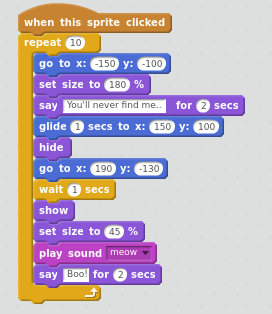
\includegraphics[scale = 0.5]{1_1}
\caption{Scratch program til delopgave 1.1}
\end{figure}

\section*{Del 1.2}













\end{document}



